\documentclass{article}
\usepackage{hyperref}
\usepackage{xcolor}
\usepackage{enumitem}
\usepackage{geometry}
\usepackage{parskip}
\usepackage{graphicx}
\usepackage{tikz}
\usepackage{titlesec}
\usepackage{tcolorbox}
\usepackage{fancyhdr}
\usetikzlibrary{mindmap,trees}
\usepackage{array}
\usepackage[T1]{fontenc}
\usepackage{lmodern}

\definecolor{feugreen}{HTML}{1C5310}
\definecolor{feuyellow}{HTML}{FDB813}
\definecolor{feulightgreen}{HTML}{2E7D32}
\definecolor{feugold}{HTML}{FFD700}

\geometry{
    a4paper,
    top=3cm,
    bottom=2.5cm,
    left=2.5cm,
    right=2.5cm,
    headheight=25pt
}

\pagestyle{fancy}
\fancyhf{}
\fancyhead[L]{\color{feugreen}GED0001 - Specialized English Program}
\fancyhead[R]{\color{feugreen}Far Eastern University}
\fancyfoot[C]{\color{feugreen}\thepage}
\renewcommand{\headrulewidth}{1pt}
\renewcommand{\headrule}{\hbox to\headwidth{\color{feugreen}\leaders\hrule height \headrulewidth\hfill}}

\titleformat{\section}
{\color{feugreen}\Large\bfseries}
{\thesection}{1em}{}[\titlerule]

\titleformat{\subsection}
{\color{feulightgreen}\large\bfseries}
{\thesubsection}{1em}{}

\newtcolorbox{feubox}{
    colback=feugreen!5,
    colframe=feugreen,
    boxrule=0.5pt,
    arc=4pt,
    boxsep=5pt,
    left=6pt,
    right=6pt,
    top=6pt,
    bottom=6pt
}

\tikzset{
    level 1/.style={
        level distance=4.5cm,
        sibling distance=4cm,
        concept color=feugreen!40
    },
    level 2/.style={
        level distance=3.5cm,
        sibling distance=2.5cm,
        concept color=feuyellow!40
    },
    every node/.style={
        align=center,
        font=\small
    }
}

\title{
    \includegraphics[width=0.6\textwidth]{FEU-with-Roman.png}\\[1cm]
    {\color{feugreen}\Huge\textbf{GED0001 Website Structure:}}\\[0.5cm]
    {\color{feulightgreen}\Large\textbf{Digital Reading Portfolio}}
}
\author{
    {\Large Far Eastern University Institute of Technology}
}
\date{
    \vspace{1cm}
    {\color{feugreen}\textbf{SPECIALIZED ENGLISH PROGRAM}}\\[0.3cm]
    {\color{feulightgreen}\textbf{FINAL EXAMINATION}}\\[0.3cm]
    {\color{feugreen}\textbf{Digital Reading Portfolio Website}}
}

\setlist[description]{
    font=\normalfont,
    style=multiline,
    leftmargin=3em,
    labelindent=0pt,
    labelwidth=2em,
    labelsep=1em,
    align=left
}

\hypersetup{
    colorlinks=true,
    linkcolor=feugreen,
    filecolor=feugreen,
    urlcolor=feugreen,
    pdftitle={Digital Reading Portfolio},
    pdfauthor={Far Eastern University},
    pdfsubject={GED0001 Website Structure},
    pdfkeywords={Digital Reading Portfolio, FEU, Technical Reading}
}

\begin{document}

\maketitle

\section*{Introduction}
We are students from Far Eastern University Institute of Technology, creating a Digital Reading Portfolio as part of our final requirement for Specialized English Program (GED0001). This portfolio showcases our development in technical reading comprehension, analysis, and critical thinking skills through various assignments and reflections. Our website serves as a comprehensive platform to demonstrate our learning journey and achievement of course outcomes.

\section*{Website Sitemap}
\begin{center}
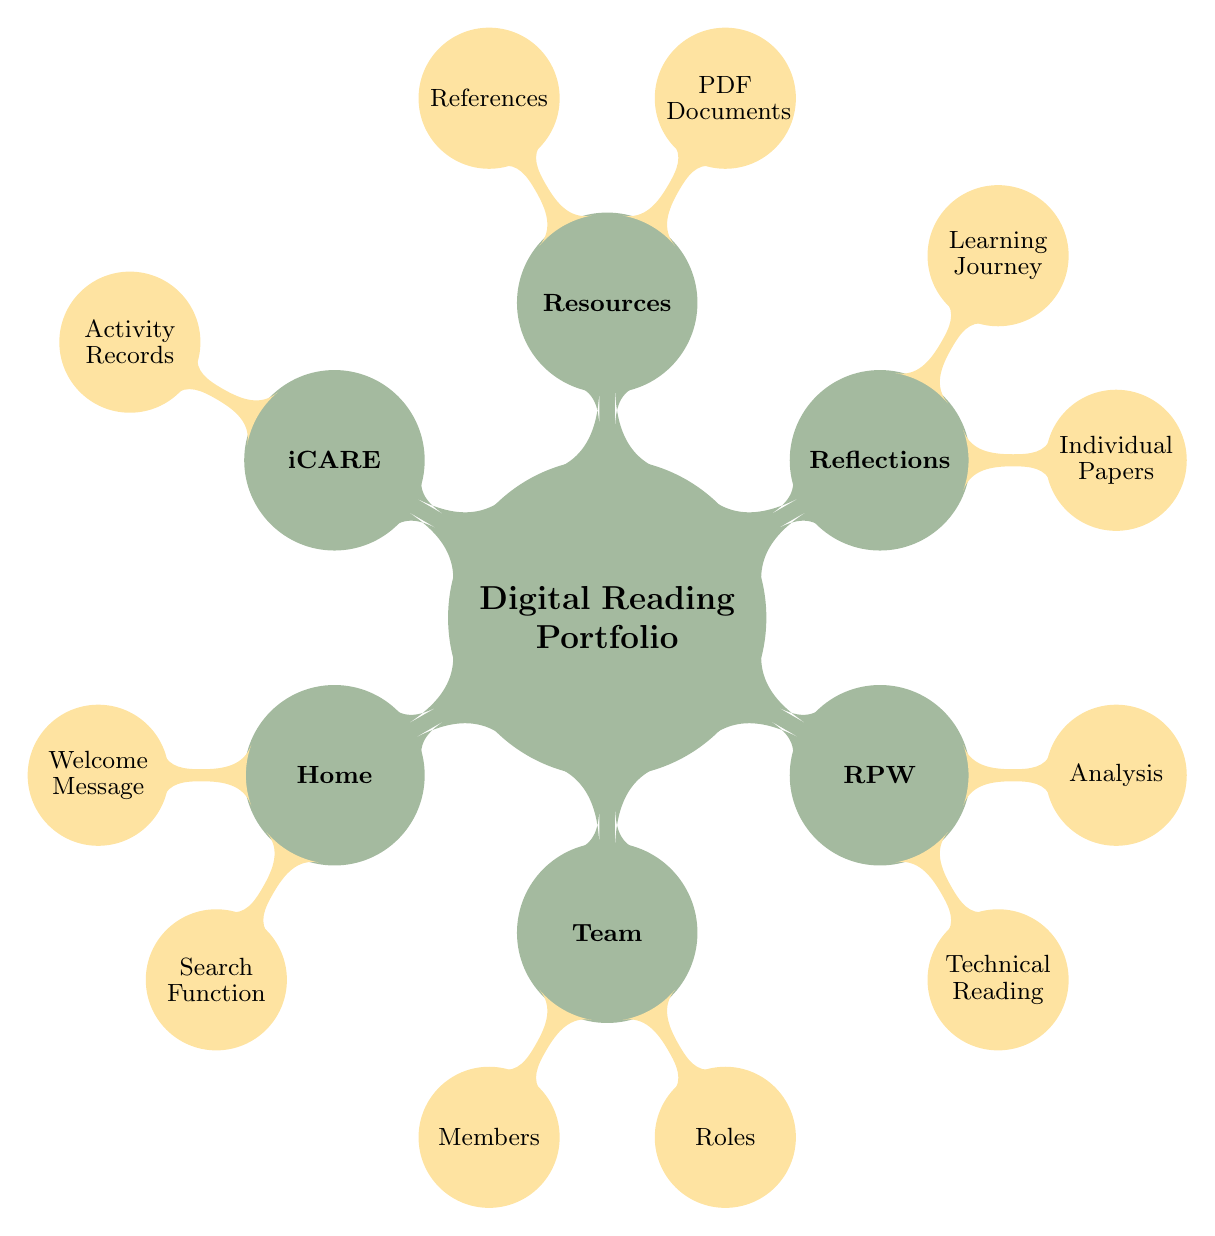
\begin{tikzpicture}[mindmap, grow cyclic, every node/.style=concept, concept color=feugreen!40,
    level 1/.append style={level distance=4cm,sibling angle=60},
    level 2/.append style={level distance=3cm}]

\node{\textbf{Digital Reading\\Portfolio}}
    child { node {\textbf{Home}}
        child { node {\small{Welcome\\Message}} }
        child { node {\small{Search\\Function}} }
    }
    child { node {\textbf{Team}}
        child { node {\small{Members}} }
        child { node {\small{Roles}} }
    }
    child { node {\textbf{RPW}}
        child { node {\small{Technical\\Reading}} }
        child { node {\small{Analysis}} }
    }
    child { node {\textbf{Reflections}}
        child { node {\small{Individual\\Papers}} }
        child { node {\small{Learning\\Journey}} }
    }
    child { node {\textbf{Resources}}
        child { node {\small{PDF\\Documents}} }
        child { node {\small{References}} }
    }
    child { node {\textbf{iCARE}}
        child { node {\small{Activity\\Records}} }
    };
\end{tikzpicture}
\end{center}

\section*{Purpose of the Website}
\subsection*{Our Mission}
To showcase our development in technical reading comprehension and analysis through an organized digital portfolio.

\subsection*{Our Goals}
\begin{itemize}[leftmargin=*]
    \item \textbf{Demonstrate Learning:} Present our understanding and analysis of technical texts
    \item \textbf{Document Growth:} Track our progress in reading comprehension and critical thinking
    \item \textbf{Showcase Skills:} Display our ability to analyze and evaluate technical materials
\end{itemize}

\section*{Website Structure}
\subsection*{1. Home Section}
\begin{description}
    \item[\textbf{Headline:}] 
    Digital Reading Portfolio: Showcasing Technical Reading Excellence
    \item[\textbf{Subheadline:}] 
    A project by FEU Tech students for GED0001 - Specialized English Program
    \item[\textbf{Features:}]
    \begin{itemize}[label={--}]
        \item Welcome message
        \item Quick navigation menu
        \item Search functionality
    \end{itemize}
\end{description}

\section*{Team Members and Roles}
\begin{feubox}
\begin{tabular}{p{3cm}p{8cm}}
\textbf{Role} & \textbf{Name} \\
\hline
Team Leader & Pantaleon, Hannah Coleen D. \\
Web Developer & Manalo, Angelo \\
Content Writers & Castro, Christian Aaron \\
& Cantuba, Maruel Zoe \\
& Tabago, Marc Alexis \\
& Cruz, Jan Mychal \\
& Suarez, Ken Enrique \\
& Cachuela, Maricar Joi
\end{tabular}
\end{feubox}

\subsection*{2. Reading Process Worksheets (RPW)}
\textbf{Content:}
\begin{itemize}
    \item \textbf{Technical Reading Analysis:}
    \begin{itemize}
        \item "Are We Too Dependent on Technology?" analysis
        \item Vocabulary development
        \item Critical evaluation
    \end{itemize}
    \item Interactive PDF viewer with annotation capabilities
    \item Structured analysis worksheets
\end{itemize}

\subsection*{3. Reflection Papers}
\textbf{Content:}
\begin{itemize}
    \item Individual reflection papers from team members
    \item Professional development documentation
    \item Learning journey narratives
    \item Course outcome achievement evidence
\end{itemize}

\section*{Technical Implementation}
\begin{feubox}
\begin{itemize}[leftmargin=*]
    \item \textbf{Core Features}
    \begin{itemize}
        \item Responsive PDF viewer
        \item Full-text search functionality
        \item Member profile system
        \item Mobile-friendly interface
    \end{itemize}
    
    \item \textbf{User Experience}
    \begin{itemize}
        \item Intuitive navigation
        \item Fast loading times
        \item Easy document access
        \item Clear information hierarchy
    \end{itemize}
\end{itemize}
\end{feubox}

\section*{Evaluation Criteria}
\begin{feubox}
\begin{itemize}[leftmargin=*]
    \item \textbf{Content Quality (40\%)}
    \begin{itemize}
        \item Completeness of RPW
        \item Quality of reflection papers
        \item Technical analysis depth
    \end{itemize}
    
    \item \textbf{Website Implementation (30\%)}
    \begin{itemize}
        \item Functionality
        \item User experience
        \item Technical features
    \end{itemize}
    
    \item \textbf{iCARE Activities (20\%)}
    \begin{itemize}
        \item Completion of required activities
        \item Documentation quality
    \end{itemize}
    
    \item \textbf{Presentation (10\%)}
    \begin{itemize}
        \item Professional appearance
        \item Organization
        \item Accessibility
    \end{itemize}
\end{itemize}
\end{feubox}

\end{document}
